\section{Question Selection}
\label{sec:selection}

\eat{
%Current implementations of crowdsourcing in databases such as CrowdDB \cite{DBLP:conf/sigmod/FranklinKKRX11} and Qurk \cite{DBLP:conf/sigmod/MarcusWKMM11} have focused primarily on using human computation at the query processing level, enabling human workers to fill in missing tables when the data is queried.  The query itself allocates on-line which entries should be modified by humans.  \sysName contrasts with this methodology by pre-processing the crowdsourcing portions off-line.

%The problem that results is in which entries should be sent to the crowd for modification.  The underlying data model of \sysName is a database of tokens.  We can represent each token in terms of a question posted to Mechanical Turk.  Such questions provide a token and allow workers to supply the true label of that token.  Given that large scale databases may contain millions of token entries, asking any type of large subset can become prohibitively expensive.  For instance, asking 5 Turkers per question at \$0.01 apiece, 100,000 tokens would still cost \$5,000. Therefore, it would help to limit the number of questions needed to produce a sizeable gain in accuracy of the database.
}

%The first step in the data cleaning process is to decide which relations should be formulated into questions posed to the ground.  Given a fixed budget, we want to select in a manner that maximizes the information gain of each question.  This is equivalent to maximally selecting the most informative tokens from the entire token space $\mathcal{T}$.  Our approach consists of three steps: first selecting the most informative token from each document (Seeding), then aggregating redundant tokens (Clustering), and finally ordering the set using information theory to select the \topk according to a budget.  We term the entire selection process InfoSelect and the full algorithm is displayed in Algorithm~\ref{alg:infoselect}. 
  
The problem of question selection is similar to that found in active learning where select examples are chosen from a pool of unlabeled data to be annotated based on some querying strategy.  While active learning has been applied to the sequential learning domain~\cite{Settles:2008:AAL:1613715.1613855,Cheng:2008:MMA:1425611.1425645} the financial and temporal cost of labeling an entire sequence (document) is not amenable to AMT’s microtask framework.  Additionally, we found documents to contain sparse labeling errors and annotation of an entire document represents unneeded redundancy.  

This necessitates tasks where examples can be partially labeled over specific tokens.  Since these examples cannot be used to re-train the supervised learning algorithm without a complete annotation, feedback is no longer used to improve the model, but to reduce the posterior uncertainty in the results.  By re-running inference with selected tokens constrained to their crowd-annotated values, we can drastically improve accuracy in a cost effective way that does not require the labeling of every token.

To properly select tokens, we need a way of properly assessing their \textit{information value}.  For a token $\mathbf{x_{i}}$ with labels $\mathbf{y_{i}}$, let $\phi(\mathbf{x_{i}})$ be a function that maps each token to its information value according to some strategy. A standard technique in active learning is to choose examples with the highest entropy, or for a sequence, the highest average marginal entropy of the individual nodes~\cite{Settles:2008:AAL:1613715.1613855}.  This \textbf{token entropy (TE)} is defined as
\begin{equation}
\phi^{TE}(\mathbf{x_{i}}) = -\sum_{l=1}^{L}P(y_{i}=l)logP(y_{i}=l),
\end{equation}
where the sum is over the range of labels $L$ and $P(y_{i}=l)$ is the marginal probability of token $\mathbf{x_{i}}$ given label $l$.

Token entropy quantifies the uncertainty in the prediction result for each individual token. While this method works well in practice for sequence models, the dependence properties shared between tokens increase the complexity of the selection process. Indeed, labels are not chosen greedily by their highest marginal probabilities, but using the dynamic programming Viterbi algorithm where suboptimal local choices can lead to a correct global solution.

In short, marginal probabilities and their corresponding entropy are not telling us the whole story. We develop two new techniques for maximizing the information value of tokens sent to the crowd for labeling. First, we exploit \textit{mutual information} (MI) to select those tokens whose result will have the greatest significance on its neighbors within a document.  Additionally, we use \textit{density estimation} to select tokens with the greatest redundancy across multiple documents.  These techniques have been previously studied in the active learning domain~\cite{Xu:2007:IDD:1763653.1763684,ZhaoJi} particularly for document retrieval, but to our knowledge have not been applied to a partial labeling scheme over a probabilistic sequence model.

Algorithm~\ref{alg:QuestionSelect} shows the psuedo-code for our entire selection method.  The filtering step assumes each token already has a mutual information score associated with it.  We iterate through all tokens, keeping only the maximum MI tokens for each document.  The clustering step iterates through filtered tokens, adding those with similar properties to the same cluster and creating new clusters as necessary.  The final cluster set is then sorted where the \topk may be drawn.  We now delve into each of these steps in more detail, based on a review of previous work found in~\cite{castleHcomp}.

\begin{algorithm}[fillcomment]
\label{alg:QuestionSelect}
\SetKwInOut{Input}{input}\SetKwInOut{Output}{output}
\Input{Set of all tokens $\mathcal{T}$}
\Output{Ranked set $C$ of maximum information clusters}
\BlankLine
\lnl{}Initialize selected token set $S$\;
\lnl{}Initialize cluster set $C$\;
\CommentSty{//Filtering}\;
\lnl{l:highEntStart}\ForEach{$t \in \mathcal{T}$}
{
	\lnl{}$i \leftarrow t.\text{docID}$\;	
	\lnl{}\If{$S(i) = \text{NULL}$}
	{
		\lnl{}$S(i) = t$\; 	
	}	
	\lnl{}\ElseIf{$S(i).\text{MI} < t.\text{MI}$}
	{
		\lnl{l:highEntEnd}$S(i) = t$\;
	}
}
\CommentSty{//Clustering}\;
\lnl{l:clustBegin}Load all tokens in $S$ into queue $Q$\;
\lnl{}\ForEach{$t \in Q$}
{
	\lnl{}\ForEach{cluster $c \in C$}
	{
		\lnl{}\If{$c$.text $=$ $t$.text \&\\
			$c$.label $=$ $t$.label \&\\
			$c$.prevLabel $=$ $t$.prevLabel \&\\
			$c$.postLabel $=$ $t$.postLabel}
			{
				\lnl{}Add $t$ to cluster $c$\;
				\lnl{}$c$.totalInfoGain $\leftarrow c$.totalInfoGain $+ t$.totalInfoGain\;
			}
	}
	\lnl{}\If{$t$ not added to a cluster}
	{
		\lnl{}Initialize new cluster $c$\;
		\lnl{}$c$.text $\leftarrow$ $t$.text\;
		\lnl{}$c$.label $\leftarrow$ $t$.label\;
		\lnl{}$c$.prevLabel $\leftarrow$ $t$.prevLabel\;
		\lnl{}$c$.postLabel $\leftarrow$ $t$.postLabel\;
		\lnl{}Add $c$ to cluster set $C$\;
                     \lnl{l:clustEnd}$c$.totalInfoGain $\leftarrow t$.totalInfoGain
	}
	
}
\CommentSty{//Ranking}\;
\lnl{}SORT clusters $c \in C$ by $c$.totalInfoGain\;

\caption{QuestionSelect}
\end{algorithm}


\subsection{Filtering by Mutual Information}
Mutual information (MI) is an information theoretic measure of the mutual dependence shared by two random variables
(RVs). Specifically, for two RVs $\mathcal{X}$ and $\mathcal{Y}$, the \textbf{mutual information} is defined in terms of entropy as
\begin{equation}
I(\mathcal{X};\mathcal{Y}) = H(\mathcal{X}) + H(\mathcal{Y}) - H(\mathcal{X},\mathcal{Y}).
\end{equation}
It represents the difference between the joint entropy $H(\mathcal{X};\mathcal{Y})$ and the individual entropies $H(\mathcal{X})$ and $H(\mathcal{Y})$. Intuitively, MI describes the reduction of uncertainty of one RV given knowledge of another. Random variables that are highly correlated will have small joint entropies whereas they are equivalent to the sum of individual entropies if the
variables are independent.

If we plan to run the inference algorithm over a partially labeled set, we need to determine precisely which variables will give the most information for the remaining ones in the sequence. This entails calculating the mutual information of every node against all others. The query strategy then becomes
\begin{align}
\label{eq:dqi}
\phi^{MI}(\mathbf{x_{i}}) = H(\mathbf{x_{i}}) + H(&\mathbf{x_{1}}, \dots, \mathbf{x_{n}}\backslash\mathbf{x_{i}}) \nonumber\\
                                                                                    & - H(\mathbf{x_{1}}, \dots, \mathbf{x_{n}})
\end{align}
where $H(\mathbf{x_{1}}, \dots, \mathbf{x_{n}}\backslash\mathbf{x_{i}})$ is the entropy of all nodes except for $\mathbf{x_{i}}$. This strategy is computationally expensive to perform on every node in every sequence. Instead we invoke a correlation of the data processing inequality, which states that information processed along a Markov chain cannot increase, i.e., for a chain $X \rightarrow Y \rightarrow Z$, where X, Y, Z are states in a chain.
\begin{equation}
I(X;Y) \geq I(X;Z)
\end{equation}
We approximate equation~\ref{eq:dqi} by utilizing its most informative neighbors, those just to the left and right in the chain.  The choice becomes selecting those tokens $\mathbf{x_{i}}$ likely to have the greatest impact on its most immediate neighbors $\mathbf{x_{i-1}}$ and $\mathbf{x_{i+1}}$
\begin{align}
\label{eq:MIapprx}
\phi^{MIapprx}(\mathbf{x_{i}}) &= I(\mathbf{x_{i-1}};\mathbf{x_{i}}) + I(\mathbf{x_{i}};\mathbf{x_{i+1}}) \nonumber\\
                                                     &=  H(\mathbf{x_{i-1}}) + 2H(\mathbf{x_{i}}) + H(\mathbf{x_{i+1}}) \nonumber\\
                                                     &     -H(\mathbf{x_{i-1}},\mathbf{x_{i}}) - H(\mathbf{x_{i}},\mathbf{x_{i+1}})
\end{align}
The entropies in equation~\ref{eq:MIapprx} can be efficiently computed using the \textit{forward-backward algorithm}~\cite{Rabiner89atutorial} to compute the marginal and joint probabilities, then the entropy calculated in the standard fashion.

Mutual information can be useful in determining the impact a node's observation has on other nodes within an individual sequence, but tells us nothing about the distribution of tokens across all documents. If we want to optimize our selection strategy, especially for a batched selection process, we should additionally incorporate a tokens ferquency and its uncertainty.

%\subsection{Optimization}
\eat{
%\subsubsection{Seeding}
%\textbf{Highest Marginal Entropy:} While we may sort all of the tokens in the database by entropy and select the \topk, this may lead to less than optimal results.  Individual tokens are not independent.  Given the evidence label of one token in a document may invoke additional corrections when the inference algorithm is re-run.  We discuss this constrained inference idea further in the context of data integration in Section~\ref{sec:integration}.  Suffice to say, because of complex probabilistic dependencies between tokens in a document, we choose to only select one token per document for the time being.  This is justified by Figure~\ref{fig:ent_dist}, which shows the entropy distribution for a typical document.  The highest entropy values appear in isolated neighborhoods which correspond to the segmentation boundaries.  The first large peak is the boundary between the Title and Author fields, with two smaller peaks illustrating additional field boundaries.  Since constrained inference primarily supplies additional correction the neighborhoods of constrained tokens, the probability of two selected tokens sharing the same "correction window" is high and the best choice is to choose a single token for each batch of questions.

%Referring again to Algorithm~\ref{alg:infoselect}, the explicit process can be found in lines~\ref{l:highEntStart}-\ref{l:highEntEnd}.  All tokens are cycled through linearly.  If the token is the first one seen from its document, it's selected.  Additional tokens from the same document are compared by marginal entropy and replaced if the new token's entropy is greater than the old one.  For the remainder of this discussion we refer to selection of a token and selection of document interchangeably.



%\noindent\textbf{Highest Marginal Neighborhood Entropy:} One drawback to selecting tokens by highest marginal entropy is that it doesn't take advantage of correlations that exist between tokens.  An optimization to the marginal entropy approach is to define entropy in a new manner as the average marginal among all of its neighbors, which we coin the \textit{marginal neighborhood entropy},

\begin{equation}
H_{n}(\mathbf{X}_{i}) = \frac{1}{3}\left(H(\mathbf{X}_{i-1}) + H(\mathbf{X}_{i}) + H(\mathbf{X}_{i+1})\right).
\end{equation}

%For a linear-chain CRF we average among the token and its left and right neighbors, but the size of the neighborhood could vary among more complex CRFs.  While we omit the proof here, it's straightforward to see that the relationship in Equation~\ref{eq:condEnt} holds for this new form of entropy.  As before, the selection process for each document becomes one of selecting the token with the maximum marginal neighborhood entropy and so long as this value replaces the traditional entropy calculation, the pseudo-code in Algorithm~\ref{alg:infoselect} remains unchanged.  We compare the two entropy definitions in the Section~\ref{sec:experiments}.
}

\begin{figure*}[t]
		\centering
		\subfigure[]{
			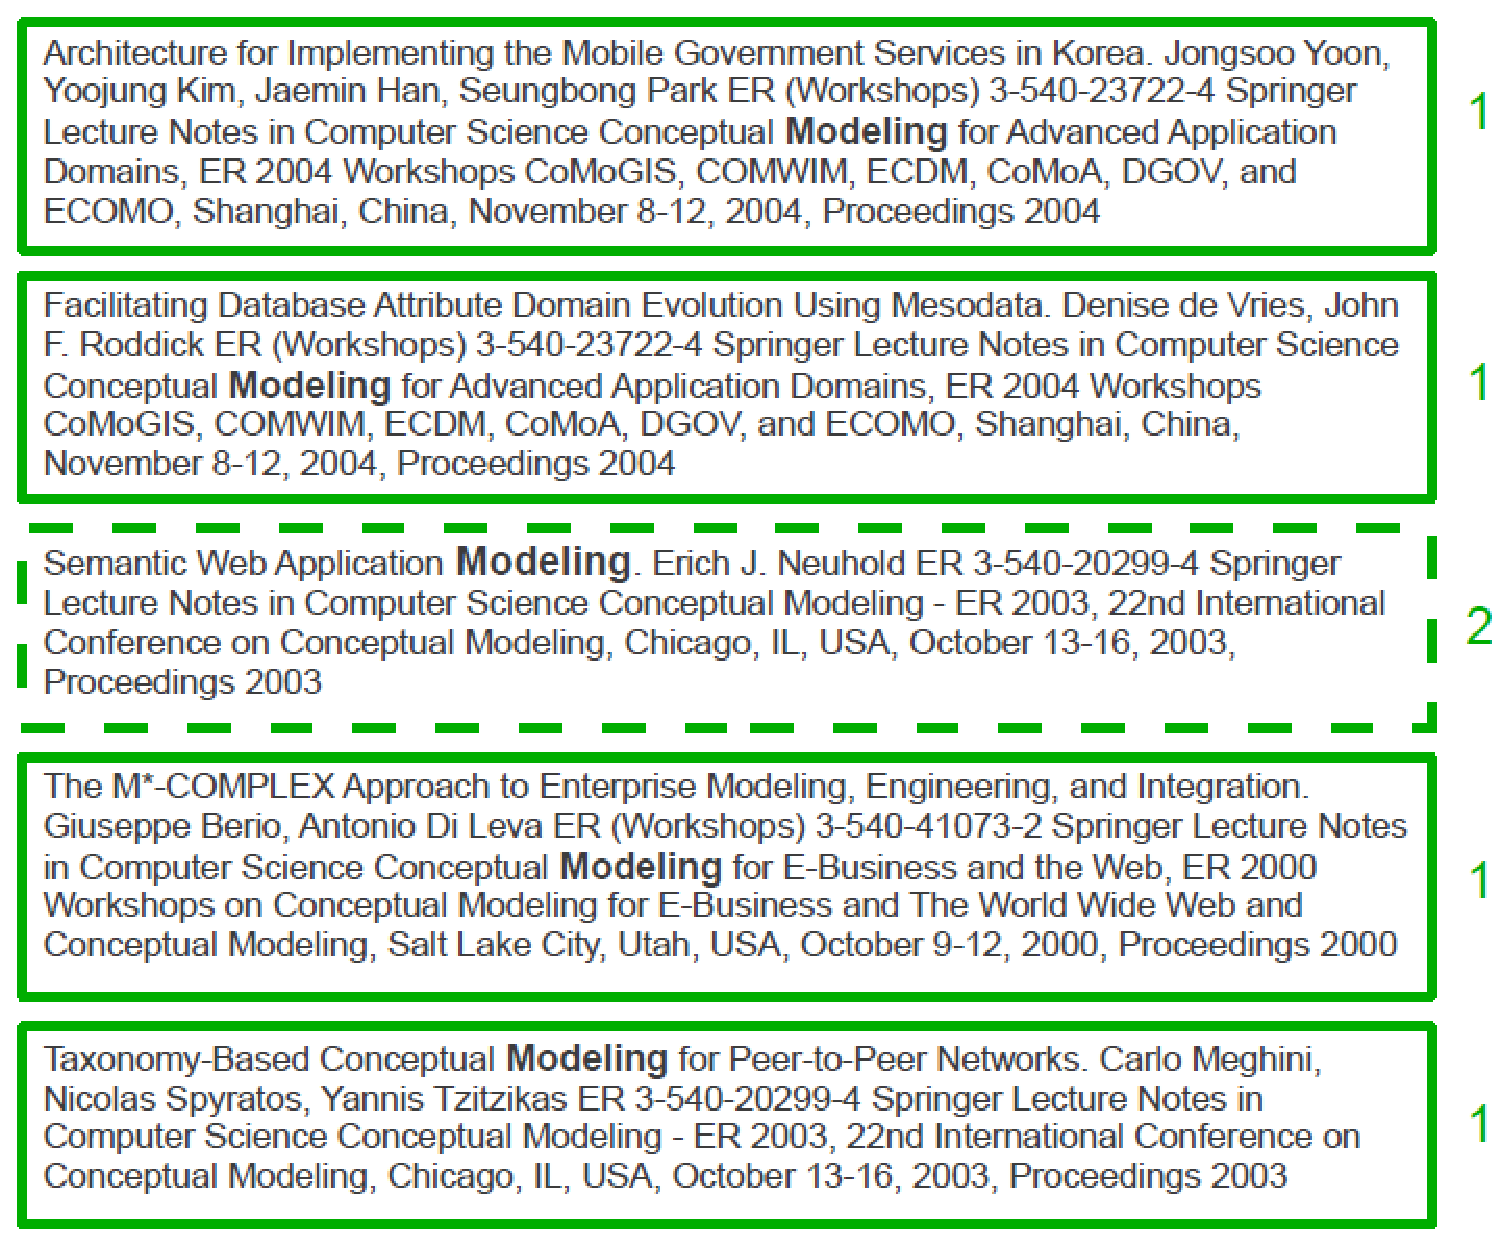
\includegraphics[width=0.47\textwidth]{cluster2.eps}
			\label{fig:token}
		}
		\subfigure[]{
			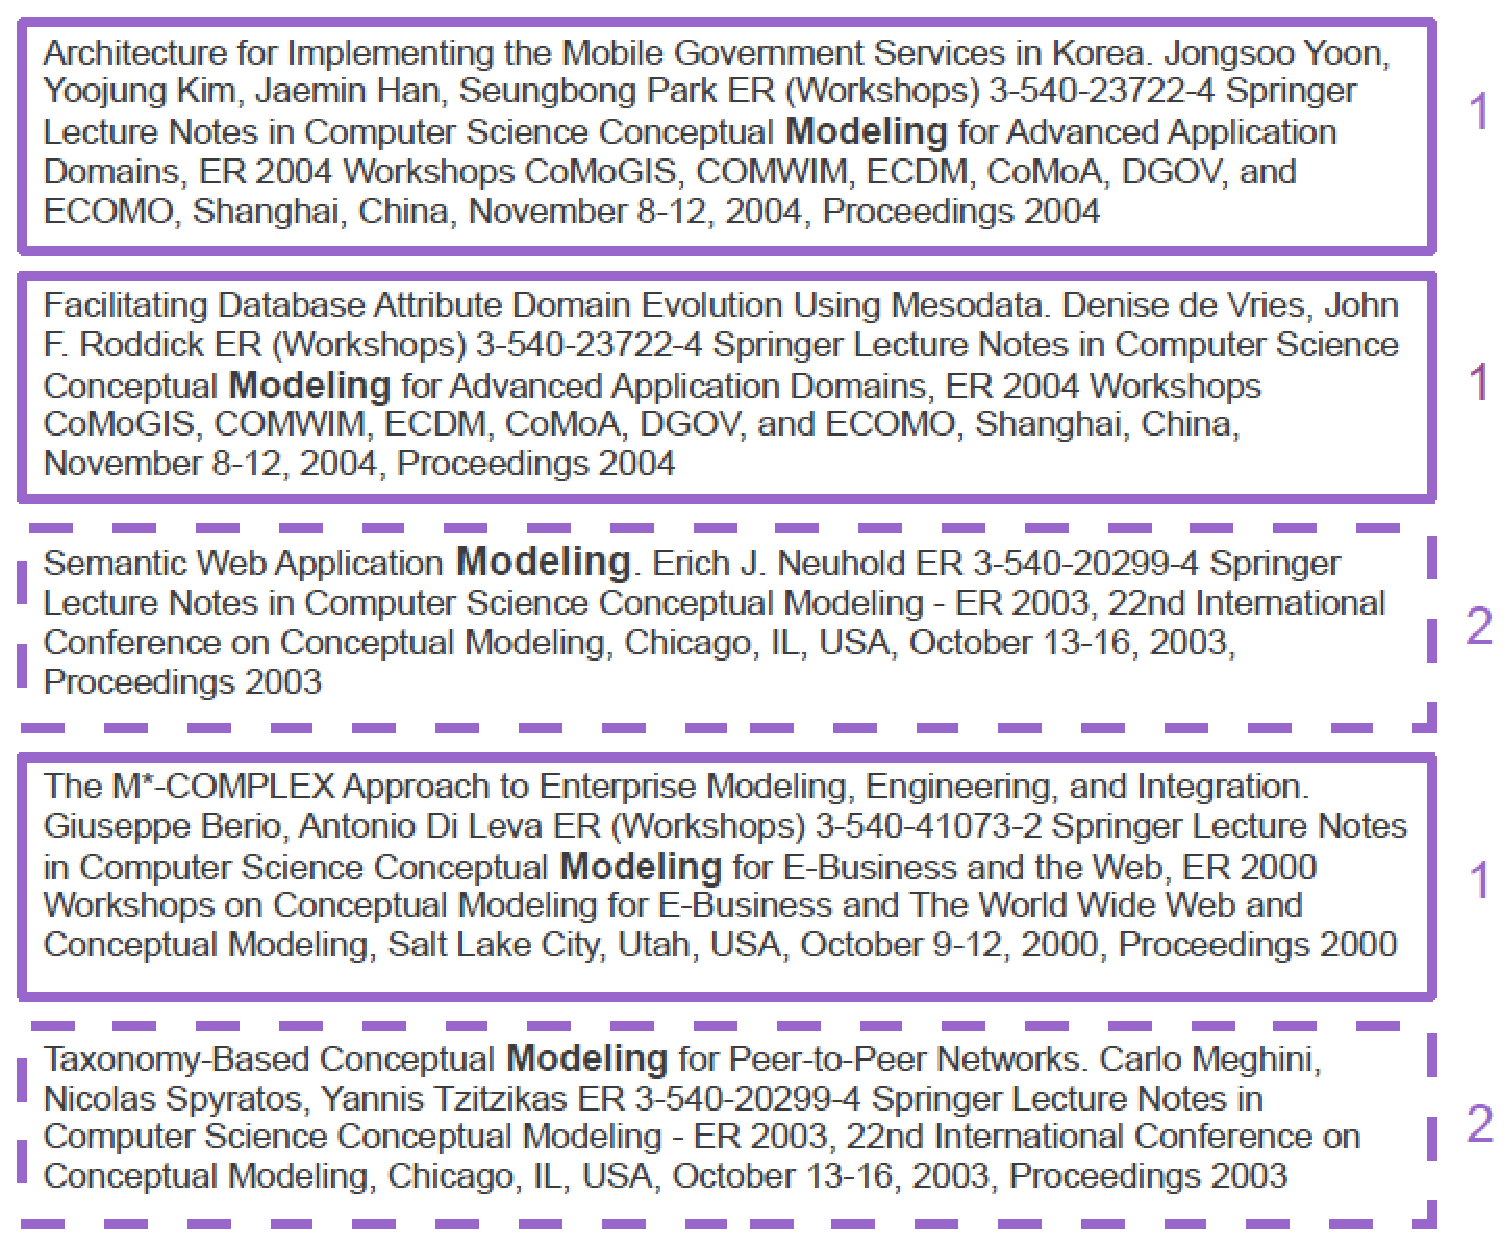
\includegraphics[width=0.47\textwidth]{cluster3.eps}
			\label{fig:label}
		}
		\caption{Clustering for the token ``Modeling'' shown over five example citations with each line type denoting a different cluster.  The level of clustering and error rate differ among whether (a) token trigrams or (b) label trigrams are used for clustering.} 
		\label{fig:cluster}
\end{figure*}

\subsection{Clustering by Information Density}

A major efficiency drawback to many active learning schemes is that they are myopic. An instance is selected
for labeling, the model is re-trained, and the process is iteratively repeated. The iterative method fails to harness the parallelizability of the crowd ecosystem. Alternativley, the faculty select tokens in batch and query the crowd at once rather than in a sequential manner. One factor that can compromise effectiveness is if there are similar token instances in the batch, as querying the label of two similar instances is equivalent to querying either of them and applying the label to both. 

We propose a scheme to cluster those tokens that should be labeled similarly and address two key issues. First, final batch must be \textit{diverse} and contain only one token from each cluster. The batch must also be \textit{dense} and contain the largest clusters whose labeling will have the greatest effect.  

In order to cluster tokens appropriately, we must define a meaningful similarity measure between them. A naive approach would cluster strictly those tokens which are equivalently out of context. This is less than desirable in our text segmentation scenario where location of the token in the document matters. Context is also important in other IE problems such as named entity recognition (NER) where homonyms with different meanings and subsequent labelings would be incorrectly grouped together.

Thus we are led to consider a \textbf{token trigram} clustering model, where tokens with similar neighbors are clustered together. Let $\mathbf{x_{i}}$ be a token at position $i$ in some document.  Together with its left and right neighbors we form the trigram $(\mathbf{x_{i-1}},\mathbf{x_{i}},\mathbf{x_{i+1}})$.  Despite being clustered as a trigram, the selection process selects the single middle token to query the crowd. We take the intuitive assumption that middle tokens $\mathbf{x_{i}}$ belonging to the same trigram are highly likely to share the same context and ought to be labeled the same. For each trigram cluster in the corpus, a single ``representative token'' with the highest mutual information (or token entropy) is selected and crowd-annotation applied to all the middle tokens in the cluster. Figure~\ref{fig:token} shows an example token trigram clustering.  

In domains such as bibliographic citation IE, many-token phrases such as common proceedings names and conference locations appear throughout multiple documents.  Common trigrams when compared across all tokens, however, are relatively infrequent. The token trigram model produces very few classification errors, but non-singleton clusters are very sparse.

There is more to the notion of context than just duplicate words appearing together. Words used in a similar ``sense" and likely to share the same label may use many different words which contextually mean the same thing. There are many ways to label how a word is used that form the fundamental backbone of NLP annotation tags, such as part-of-speech (POS), entity tags, segmentation tags, dependency parses, etc.

A token $\mathbf{x_{i}}$ has a set of associated labels $\mathbf{l_{i,j}}$, where $i$ again denotes label position and $j$ some numerical representation of the classifier type. For example, $\mathbf{l_{i,0}}$ might be the POS tag associated with $\mathbf{x_{i}}$ while $\mathbf{l}_{i,1}$ might be a segmentation tag. A \textbf{label trigram} clustering model consists of tokens that share some specified set of label trigrams. One possible cluster would be $(\mathbf{x_{i}}, (\mathbf{l_{i-1,1}},\mathbf{l_{i,1}},\mathbf{l_{i+1,1}}))$, which groups individual tokens labeled with the same segmentation tag and sharing left and right neighbors labeled the same. One requirement for all label trigram clusters is that that the individual tokens$\mathbf{x_{i}}$ should still be the same. Figure~\ref{fig:label} illustrates an example of label trigram clustering.

While these labels are themselves the uncertain output of machine learning classifers, our experiments show contextually similar tokens are also similarly mislabeled and still cluster appropriately. Overall, the label trigram model increases the recall and amount of clustering, but at the expense of a greater rate of classification error compared to the token trigram model.

Both trigram models correspond to a mapping of tokens to a lower dimensional space where tokens sharing the same trigram properties are mapped to the same point. Selecting the largest token clusters is equivalent to selecting the ``highest density" instances according to the data distribution, a technique that has shown positive yield in traditional active learning~\cite{Guo:2007:OAL:1625275.1625408}.

\eat{
\subsubsection{Clustering}
\eat{
%Individual documents, especially citation data, may contain significant overlap between authors, conferences, publishers, etc. that appear in more than one document.  While we accept a certain redundancy for quality control purposes, this should be tightly controlled through the AMT interface.  Selecting the same tokens with the same labels from different documents essentially doubles the cost for a single answer.
}

%The next optimization in the selection process is to eliminate redundant tokens in $S$. The same authors, conferences, years, etc. may be shared across multiple documents and not all tokens in $S$ may be unique.  For maximum information gain, we constrain the token set further to a set of unique tokens $R \subseteq S$.  All non-unique tokens are clustered together and single one chosen to be that cluster's \textit{representative}.  It is the representative's full document context which is sent to the crowd and the answer received is applied to all tokens in the cluster.  This allows a many-to-one relationship to exist between tokens and questions.  The choice of cluster representative is arbitrary and here we take it to be the token with the highest entropy. 

%The problem is finding such a set of representative clusters $R \subseteq S$ so that only $R$ questions need be asked to entirely cover the space of $S$.  The naive approach to clustering would be to define tokens with the same string text as being similar.  This can lead to inaccuracies for generic words.  For example, the word "computer" may appear in multiple contexts such as the title on "Human-Computer Interaction" or in a journal like "Lecture Notes in Computer Science".  See Figure~\ref{fig:cluster} for additional examples.

%We define a number of \textit{cluster properties} to ensure all tokens in a cluster should indeed be mapped to the same label.  There is a balance to be had between the size of the cluster and their accuracies.  The larger the clusters the greater impact each individual question has.  At one end of the extreme, we can group everything into one cluster so that $|R| = 1$.  Cost would be optimized, but at the expense of many mislabeled tokens.  On the other hand, everything can be grouped as a singleton so that $|R| = |S|$.  The clustering accuracy will be 100\%, but at a greater cost.  We want to define clusters in such a way that we balance between these two extremes and group tokens accurately, but not stringently, so that large clusters may develop.  In some cases, we can allow some leniency in misclustering if it's balanced out large improvement among correct clusterings.  Below we describe three sets of properties in order of decreasing selectivity of cluster admission.  The clustering process in Algorithm~\ref{alg:infoselect} is contained in lines~\ref{l:clustBegin} and~\ref{l:clustEnd} for the example set of \text{same label neighborhood} properties.


\eat{
%Our solution to this problem is through a novel clustering technique.  Tokens that share similar text and machine labeling properties have a high probability of sharing the same true labels.  By mapping multiple tokens into the same \textit{Question Cluster}, a single answer can be used to modify labels for a large number of tokens.  Whereas before we constrained the token space to the set of documents, here we constrain the space even further to only the set of unique clusters.  In the rest of this section we describe three specific cluster sets of cluster properties.

%All cluster sets require tokens belonging to the cluster to share the same token text and machine labeling, but are set apart by different neighborhood constraints.  Context is important because it's possible that two tokens with the same text such as the word "computer" could actually require different labelings and it would be false to cluster them together.  The different cluster properties trade off accuracy and cluster size and we compare them in the experiments section.  Figure~\ref{fig:cluster} compares two similar tokens and illustrates the different cluster properties that are checked.
}

%\textbf{Same Field:} The strictest of the cluster properties.  It promotes the least amount of clustering, but adheres to greatest accuracy.  The initial cluster representative defines a field by its CRF max likelihood label and all preceeding and suceeding tokens with the same label as determined by the CRF model.  Tokens are only added to the cluster if they share the entire field.  Figure~\ref{fig:field} shows an example set of five citations clustered using the Same Field method for the token \textit{Modeling}.  The first two citations share the same Proceedings field and are thus clustered together.  Whichever use of \textit{Modeling} has the highest entropy for each cluster will be that token's cluster representative.

%\textbf{Same Token Neighborhood:} The simplest of the cluster properties.  We don't check any of the machine labelings, but measure redundancy based purely on the text associated with each token.  Tokens are clustered together that share the same token as well as the same token directly preceeding and suceeding it.  This has the advantage of being purely dependent on the data and not at all on the CRF output.  This approach is slightly more error-prone.  Figure~\ref{fig:token}, which clusters by the trigram \textit{Conceptual Modeling for} shows the additional clustering that can result from this method as well as the increased possibility for error, as evinced in the final citation being incorrectly clustered with the others.

%\textbf{Same Label Neighbhorhood:} A relaxing of the Same Field properties to only compare labels one position before and after the token.  The existence of sub-entities such as a city that appears in more than one Proceedings field or an author that appears with different groups of authors motivate this approach of not checking the entire field.  Clustering is greatly increased, but at the expense of a small increase in misclassification compared to the other methods.  This is partly due to its added reliance on the machine's classification, which can contain errors.  Figure~\ref{fig:label} shows what would be expected to be a correct clustering for the token \textit{Modeling}, with cluster 1 containing those entries appearing in a Proceedings and cluster 2 those appearing in a Title.
}
\subsection{Ranking by Total Information Gain}

%Given a budget of $K < |R|$ questions, the final step is to impose a total ordering upon the set $R$ and select the top $K$.  We consider three different ways of ordering clusters for selection: by highest representative entropy, by cluster size, and by total cluster entropy.  Again, by equation~\ref{eq:condEnt}, our total utility function $H(\mathbf{Y}|\mathbf{X})$ at each step is minimized by selecting the token with the maximum marginal entropy.  We can thus order the tokens in $R$ by one at a time selecting the cluster representative with the highest entropy.  This type of ordering is ideal for applications with numerous small clusters.  For larger clusters, more information may be gained by ordering by cluster size to ensure the largest number of total tokens are covered by the budget.  For comparison, we also consider a heuristic ranking that orders by the total entropy of all tokens in a cluster, striking a balance between token marginal entropy and cluster size.  The final line of Algorithm~\ref{alg:infoselect} illustrates sorting by this metric as an example.  The various orderings are compared in our experiments in Section~\ref{sec:experiments}.

Given a limited budget of questions, clusters should be ranked to facilitate selection of the \topk.  We experimented with three different ranking schemes: ranking by mutual information score of a cluster's representative token, ranking by cluster size, and ranking by total information gain.  We define the total information gain of a cluster to be the sum of all mutual information scores of all tokens that belong to a cluster.  A comparison of the three ranking approaches can be found with the experiments in Section~\ref{sec:experiments}.
\eat{
%Adhering to our information theoretic framework, it's possible to select the "representative" high entropy token used to initiate each cluster and rank by that token's individual entropy.  On the other hand, if clusters are largely skewed in size, it may be more beneficial to rank by the actual size of the cluster.  As a final heuristic attempting to combine both the entropy and cluster size approaches, we can sort by the total entropy of each cluster, that is, the sum of entropies of every token in the cluster.  Our experiments compare and contrast these different ordering techniques.
}
